\documentclass[1p]{elsarticle_modified}
%\bibliographystyle{elsarticle-num}

%\usepackage[colorlinks]{hyperref}
%\usepackage{abbrmath_seonhwa} %\Abb, \Ascr, \Acal ,\Abf, \Afrak
\usepackage{amsfonts}
\usepackage{amssymb}
\usepackage{amsmath}
\usepackage{amsthm}
\usepackage{scalefnt}
\usepackage{amsbsy}
\usepackage{kotex}
\usepackage{caption}
\usepackage{subfig}
\usepackage{color}
\usepackage{graphicx}
\usepackage{xcolor} %% white, black, red, green, blue, cyan, magenta, yellow
\usepackage{float}
\usepackage{setspace}
\usepackage{hyperref}

\usepackage{tikz}
\usetikzlibrary{arrows}

\usepackage{multirow}
\usepackage{array} % fixed length table
\usepackage{hhline}

%%%%%%%%%%%%%%%%%%%%%
\makeatletter
\renewcommand*\env@matrix[1][\arraystretch]{%
	\edef\arraystretch{#1}%
	\hskip -\arraycolsep
	\let\@ifnextchar\new@ifnextchar
	\array{*\c@MaxMatrixCols c}}
\makeatother %https://tex.stackexchange.com/questions/14071/how-can-i-increase-the-line-spacing-in-a-matrix
%%%%%%%%%%%%%%%

\usepackage[normalem]{ulem}

\newcommand{\msout}[1]{\ifmmode\text{\sout{\ensuremath{#1}}}\else\sout{#1}\fi}
%SOURCE: \msout is \stkout macro in https://tex.stackexchange.com/questions/20609/strikeout-in-math-mode

\newcommand{\cancel}[1]{
	\ifmmode
	{\color{red}\msout{#1}}
	\else
	{\color{red}\sout{#1}}
	\fi
}

\newcommand{\add}[1]{
	{\color{blue}\uwave{#1}}
}

\newcommand{\replace}[2]{
	\ifmmode
	{\color{red}\msout{#1}}{\color{blue}\uwave{#2}}
	\else
	{\color{red}\sout{#1}}{\color{blue}\uwave{#2}}
	\fi
}

\newcommand{\Sol}{\mathcal{S}} %segment
\newcommand{\D}{D} %diagram
\newcommand{\A}{\mathcal{A}} %arc


%%%%%%%%%%%%%%%%%%%%%%%%%%%%%5 test

\def\sl{\operatorname{\textup{SL}}(2,\Cbb)}
\def\psl{\operatorname{\textup{PSL}}(2,\Cbb)}
\def\quan{\mkern 1mu \triangleright \mkern 1mu}

\theoremstyle{definition}
\newtheorem{thm}{Theorem}[section]
\newtheorem{prop}[thm]{Proposition}
\newtheorem{lem}[thm]{Lemma}
\newtheorem{ques}[thm]{Question}
\newtheorem{cor}[thm]{Corollary}
\newtheorem{defn}[thm]{Definition}
\newtheorem{exam}[thm]{Example}
\newtheorem{rmk}[thm]{Remark}
\newtheorem{alg}[thm]{Algorithm}

\newcommand{\I}{\sqrt{-1}}
\begin{document}

%\begin{frontmatter}
%
%\title{Boundary parabolic representations of knots up to 8 crossings}
%
%%% Group authors per affiliation:
%\author{Yunhi Cho} 
%\address{Department of Mathematics, University of Seoul, Seoul, Korea}
%\ead{yhcho@uos.ac.kr}
%
%
%\author{Seonhwa Kim} %\fnref{s_kim}}
%\address{Center for Geometry and Physics, Institute for Basic Science, Pohang, 37673, Korea}
%\ead{ryeona17@ibs.re.kr}
%
%\author{Hyuk Kim}
%\address{Department of Mathematical Sciences, Seoul National University, Seoul 08826, Korea}
%\ead{hyukkim@snu.ac.kr}
%
%\author{Seokbeom Yoon}
%\address{Department of Mathematical Sciences, Seoul National University, Seoul, 08826,  Korea}
%\ead{sbyoon15@snu.ac.kr}
%
%\begin{abstract}
%We find all boundary parabolic representation of knots up to 8 crossings.
%
%\end{abstract}
%\begin{keyword}
%    \MSC[2010] 57M25 
%\end{keyword}
%
%\end{frontmatter}

%\linenumbers
%\tableofcontents
%
\newcommand\colored[1]{\textcolor{white}{\rule[-0.35ex]{0.8em}{1.4ex}}\kern-0.8em\color{red} #1}%
%\newcommand\colored[1]{\textcolor{white}{ #1}\kern-2.17ex	\textcolor{white}{ #1}\kern-1.81ex	\textcolor{white}{ #1}\kern-2.15ex\color{red}#1	}

{\Large $\underline{11a_{305}~(K11a_{305})}$}

\setlength{\tabcolsep}{10pt}
\renewcommand{\arraystretch}{1.6}
\vspace{1cm}\begin{tabular}{m{100pt}>{\centering\arraybackslash}m{274pt}}
\multirow{5}{120pt}{
	\centering
	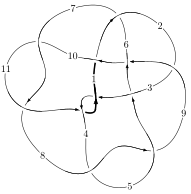
\includegraphics[width=112pt]{../../../GIT/diagram.site/Diagrams/png/554_11a_305.png}\\
\ \ \ A knot diagram\footnotemark}&
\allowdisplaybreaks
\textbf{Linearized knot diagam} \\
\cline{2-2}
 &
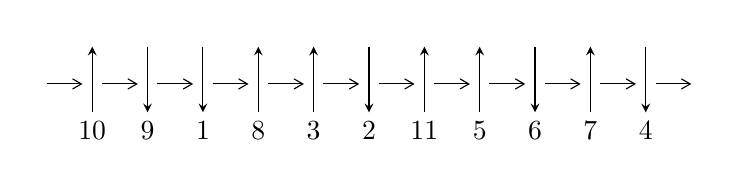
\begin{tikzpicture}[x=20pt, y=17pt]
	% nodes
	\node (C0) at (0, 0) {};
	\node (C1) at (1, 0) {};
	\node (C1U) at (1, +1) {};
	\node (C1D) at (1, -1) {10};

	\node (C2) at (2, 0) {};
	\node (C2U) at (2, +1) {};
	\node (C2D) at (2, -1) {9};

	\node (C3) at (3, 0) {};
	\node (C3U) at (3, +1) {};
	\node (C3D) at (3, -1) {1};

	\node (C4) at (4, 0) {};
	\node (C4U) at (4, +1) {};
	\node (C4D) at (4, -1) {8};

	\node (C5) at (5, 0) {};
	\node (C5U) at (5, +1) {};
	\node (C5D) at (5, -1) {3};

	\node (C6) at (6, 0) {};
	\node (C6U) at (6, +1) {};
	\node (C6D) at (6, -1) {2};

	\node (C7) at (7, 0) {};
	\node (C7U) at (7, +1) {};
	\node (C7D) at (7, -1) {11};

	\node (C8) at (8, 0) {};
	\node (C8U) at (8, +1) {};
	\node (C8D) at (8, -1) {5};

	\node (C9) at (9, 0) {};
	\node (C9U) at (9, +1) {};
	\node (C9D) at (9, -1) {6};

	\node (C10) at (10, 0) {};
	\node (C10U) at (10, +1) {};
	\node (C10D) at (10, -1) {7};

	\node (C11) at (11, 0) {};
	\node (C11U) at (11, +1) {};
	\node (C11D) at (11, -1) {4};
	\node (C12) at (12, 0) {};

	% arrows
	\draw[->,>={angle 60}]
	(C0) edge (C1) (C1) edge (C2) (C2) edge (C3) (C3) edge (C4) (C4) edge (C5) (C5) edge (C6) (C6) edge (C7) (C7) edge (C8) (C8) edge (C9) (C9) edge (C10) (C10) edge (C11) (C11) edge (C12) ;	\draw[->,>=stealth]
	(C1D) edge (C1U) (C2U) edge (C2D) (C3U) edge (C3D) (C4D) edge (C4U) (C5D) edge (C5U) (C6U) edge (C6D) (C7D) edge (C7U) (C8D) edge (C8U) (C9U) edge (C9D) (C10D) edge (C10U) (C11U) edge (C11D) ;
	\end{tikzpicture} \\
\hhline{~~} \\& 
\textbf{Solving Sequence} \\ \cline{2-2} 
 &
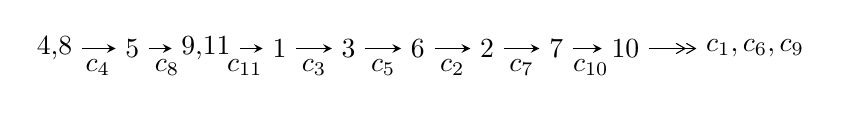
\begin{tikzpicture}[x=25pt, y=7pt]
	% node
	\node (A0) at (-1/8, 0) {4,8};
	\node (A1) at (1, 0) {5};
	\node (A2) at (33/16, 0) {9,11};
	\node (A3) at (25/8, 0) {1};
	\node (A4) at (33/8, 0) {3};
	\node (A5) at (41/8, 0) {6};
	\node (A6) at (49/8, 0) {2};
	\node (A7) at (57/8, 0) {7};
	\node (A8) at (65/8, 0) {10};
	\node (C1) at (1/2, -1) {$c_{4}$};
	\node (C2) at (3/2, -1) {$c_{8}$};
	\node (C3) at (21/8, -1) {$c_{11}$};
	\node (C4) at (29/8, -1) {$c_{3}$};
	\node (C5) at (37/8, -1) {$c_{5}$};
	\node (C6) at (45/8, -1) {$c_{2}$};
	\node (C7) at (53/8, -1) {$c_{7}$};
	\node (C8) at (61/8, -1) {$c_{10}$};
	\node (A9) at (10, 0) {$c_{1},c_{6},c_{9}$};

	% edge
	\draw[->,>=stealth]	
	(A0) edge (A1) (A1) edge (A2) (A2) edge (A3) (A3) edge (A4) (A4) edge (A5) (A5) edge (A6) (A6) edge (A7) (A7) edge (A8) ;
	\draw[->>,>={angle 60}]	
	(A8) edge (A9);
\end{tikzpicture} \\ 

\end{tabular} \\

\footnotetext{
The image of knot diagram is generated by the software ``\textbf{Draw programme}" developed by Andrew Bartholomew(\url{http://www.layer8.co.uk/maths/draw/index.htm\#Running-draw}), where we modified some parts for our purpose(\url{https://github.com/CATsTAILs/LinksPainter}).
}\phantom \\ \newline 
\centering \textbf{Ideals for irreducible components\footnotemark of $X_{\text{par}}$} 
 
\begin{align*}
I^u_{1}&=\langle 
128458353823909 u^{26}+129748020078821 u^{25}+\cdots+71455439122482 b-307532868153053,\\
\phantom{I^u_{1}}&\phantom{= \langle  }a-1,\;u^{27}-15 u^{25}+\cdots+8 u+1\rangle \\
I^u_{2}&=\langle 
6.23874\times10^{124} u^{53}+1.39776\times10^{125} u^{52}+\cdots+4.41978\times10^{127} b+4.69540\times10^{127},\\
\phantom{I^u_{2}}&\phantom{= \langle  }5.28258\times10^{127} u^{53}-1.64275\times10^{127} u^{52}+\cdots+8.57438\times10^{129} a+7.90543\times10^{128},\\
\phantom{I^u_{2}}&\phantom{= \langle  }2 u^{54}-3 u^{53}+\cdots+95 u-97\rangle \\
I^u_{3}&=\langle 
2 u^7-3 u^6-5 u^5+6 u^4+10 u^3-12 u^2+b- u+4,\;a+1,\;u^8- u^7-3 u^6+2 u^5+6 u^4-4 u^3-3 u^2+2 u+1\rangle \\
I^u_{4}&=\langle 
u^2+b,\;a+1,\;u^3- u-1\rangle \\
I^u_{5}&=\langle 
b+1,\;a-2,\;2 u-1\rangle \\
I^u_{6}&=\langle 
b+1,\;2 a-1,\;u+1\rangle \\
I^u_{7}&=\langle 
b+1,\;a+1,\;u+1\rangle \\
\\
\end{align*}
\raggedright * 7 irreducible components of $\dim_{\mathbb{C}}=0$, with total 95 representations.\\
\footnotetext{All coefficients of polynomials are rational numbers. But the coefficients are sometimes approximated in decimal forms when there is not enough margin.}
\newpage
\renewcommand{\arraystretch}{1}
\centering \section*{I. $I^u_{1}= \langle 1.28\times10^{14} u^{26}+1.30\times10^{14} u^{25}+\cdots+7.15\times10^{13} b-3.08\times10^{14},\;a-1,\;u^{27}-15 u^{25}+\cdots+8 u+1 \rangle$}
\flushleft \textbf{(i) Arc colorings}\\
\begin{tabular}{m{7pt} m{180pt} m{7pt} m{180pt} }
\flushright $a_{4}=$&$\begin{pmatrix}1\\0\end{pmatrix}$ \\
\flushright $a_{8}=$&$\begin{pmatrix}0\\u\end{pmatrix}$ \\
\flushright $a_{5}=$&$\begin{pmatrix}1\\- u^2\end{pmatrix}$ \\
\flushright $a_{9}=$&$\begin{pmatrix}u\\- u^3+u\end{pmatrix}$ \\
\flushright $a_{11}=$&$\begin{pmatrix}1\\-1.79774 u^{26}-1.81579 u^{25}+\cdots+35.4655 u+4.30384\end{pmatrix}$ \\
\flushright $a_{1}=$&$\begin{pmatrix}1.79774 u^{26}+1.81579 u^{25}+\cdots-35.4655 u-3.30384\\-1.79774 u^{26}-1.81579 u^{25}+\cdots+35.4655 u+4.30384\end{pmatrix}$ \\
\flushright $a_{3}=$&$\begin{pmatrix}2.79486 u^{26}+3.00477 u^{25}+\cdots-62.0548 u-7.92538\\-0.997121 u^{26}-1.18898 u^{25}+\cdots+26.5893 u+4.62154\end{pmatrix}$ \\
\flushright $a_{6}=$&$\begin{pmatrix}-3.74472 u^{26}-3.04658 u^{25}+\cdots+45.3634 u+2.81681\\0.625459 u^{26}+1.07598 u^{25}+\cdots-25.4593 u-2.82772\end{pmatrix}$ \\
\flushright $a_{2}=$&$\begin{pmatrix}1.08283 u^{26}+1.65073 u^{25}+\cdots-41.4105 u-5.52428\\-1.60344 u^{26}-1.67881 u^{25}+\cdots+34.6892 u+5.66859\end{pmatrix}$ \\
\flushright $a_{7}=$&$\begin{pmatrix}- u\\1.81579 u^{26}+1.36688 u^{25}+\cdots-17.6858 u-1.79774\end{pmatrix}$ \\
\flushright $a_{10}=$&$\begin{pmatrix}- u^2+1\\-0.430865 u^{26}-0.712953 u^{25}+\cdots+19.1414 u+2.48805\end{pmatrix}$\\ \flushright $a_{10}=$&$\begin{pmatrix}- u^2+1\\-0.430865 u^{26}-0.712953 u^{25}+\cdots+19.1414 u+2.48805\end{pmatrix}$\\&\end{tabular}
\flushleft \textbf{(ii) Obstruction class $= -1$}\\~\\
\flushleft \textbf{(iii) Cusp Shapes $= \frac{110984790327346}{11909239853747} u^{26}+\frac{77302583361155}{11909239853747} u^{25}+\cdots-\frac{911733716325243}{11909239853747} u-\frac{123671657013453}{11909239853747}$}\\~\\
\newpage\renewcommand{\arraystretch}{1}
\flushleft \textbf{(iv) u-Polynomials at the component}\newline \\
\begin{tabular}{m{50pt}|m{274pt}}
Crossings & \hspace{64pt}u-Polynomials at each crossing \\
\hline $$\begin{aligned}c_{1},c_{5}\end{aligned}$$&$\begin{aligned}
&u^{27}+2 u^{26}+\cdots+8 u+2
\end{aligned}$\\
\hline $$\begin{aligned}c_{2},c_{6}\end{aligned}$$&$\begin{aligned}
&u^{27}+7 u^{25}+\cdots-3 u+1
\end{aligned}$\\
\hline $$\begin{aligned}c_{3},c_{11}\end{aligned}$$&$\begin{aligned}
&u^{27}-10 u^{26}+\cdots+172 u-16
\end{aligned}$\\
\hline $$\begin{aligned}c_{4},c_{7},c_{8}\\c_{10}\end{aligned}$$&$\begin{aligned}
&u^{27}-15 u^{25}+\cdots+8 u+1
\end{aligned}$\\
\hline $$\begin{aligned}c_{9}\end{aligned}$$&$\begin{aligned}
&u^{27}+13 u^{26}+\cdots-28 u-4
\end{aligned}$\\
\hline
\end{tabular}\\~\\
\newpage\renewcommand{\arraystretch}{1}
\flushleft \textbf{(v) Riley Polynomials at the component}\newline \\
\begin{tabular}{m{50pt}|m{274pt}}
Crossings & \hspace{64pt}Riley Polynomials at each crossing \\
\hline $$\begin{aligned}c_{1},c_{5}\end{aligned}$$&$\begin{aligned}
&y^{27}-4 y^{26}+\cdots+84 y-4
\end{aligned}$\\
\hline $$\begin{aligned}c_{2},c_{6}\end{aligned}$$&$\begin{aligned}
&y^{27}+14 y^{26}+\cdots-15 y-1
\end{aligned}$\\
\hline $$\begin{aligned}c_{3},c_{11}\end{aligned}$$&$\begin{aligned}
&y^{27}+16 y^{26}+\cdots+6320 y-256
\end{aligned}$\\
\hline $$\begin{aligned}c_{4},c_{7},c_{8}\\c_{10}\end{aligned}$$&$\begin{aligned}
&y^{27}-30 y^{26}+\cdots+34 y-1
\end{aligned}$\\
\hline $$\begin{aligned}c_{9}\end{aligned}$$&$\begin{aligned}
&y^{27}-3 y^{26}+\cdots+56 y-16
\end{aligned}$\\
\hline
\end{tabular}\\~\\
\newpage\flushleft \textbf{(vi) Complex Volumes and Cusp Shapes}
$$\begin{array}{c|c|c}  
\text{Solutions to }I^u_{1}& \I (\text{vol} + \sqrt{-1}CS) & \text{Cusp shape}\\
 \hline 
\begin{aligned}
u &= \phantom{-}0.106573 + 0.849360 I \\
a &= \phantom{-}1.00000\phantom{ +0.000000I} \\
b &= \phantom{-}0.489173 - 0.963829 I\end{aligned}
 & -0.11341 + 6.75527 I & \phantom{-}1.42209 - 7.76802 I \\ \hline\begin{aligned}
u &= \phantom{-}0.106573 - 0.849360 I \\
a &= \phantom{-}1.00000\phantom{ +0.000000I} \\
b &= \phantom{-}0.489173 + 0.963829 I\end{aligned}
 & -0.11341 - 6.75527 I & \phantom{-}1.42209 + 7.76802 I \\ \hline\begin{aligned}
u &= -0.159654 + 0.781613 I \\
a &= \phantom{-}1.00000\phantom{ +0.000000I} \\
b &= \phantom{-}0.591660 + 0.371074 I\end{aligned}
 & -1.77335 + 2.61294 I & -2.81593 - 2.10661 I \\ \hline\begin{aligned}
u &= -0.159654 - 0.781613 I \\
a &= \phantom{-}1.00000\phantom{ +0.000000I} \\
b &= \phantom{-}0.591660 - 0.371074 I\end{aligned}
 & -1.77335 - 2.61294 I & -2.81593 + 2.10661 I \\ \hline\begin{aligned}
u &= \phantom{-}0.784543\phantom{ +0.000000I} \\
a &= \phantom{-}1.00000\phantom{ +0.000000I} \\
b &= -0.832565\phantom{ +0.000000I}\end{aligned}
 & \phantom{-}0.365696\phantom{ +0.000000I} & \phantom{-}11.8450\phantom{ +0.000000I} \\ \hline\begin{aligned}
u &= \phantom{-}0.779651\phantom{ +0.000000I} \\
a &= \phantom{-}1.00000\phantom{ +0.000000I} \\
b &= \phantom{-}0.197132\phantom{ +0.000000I}\end{aligned}
 & \phantom{-}1.29249\phantom{ +0.000000I} & \phantom{-}7.75610\phantom{ +0.000000I} \\ \hline\begin{aligned}
u &= \phantom{-}1.221600 + 0.595583 I \\
a &= \phantom{-}1.00000\phantom{ +0.000000I} \\
b &= \phantom{-}0.114881 - 1.150240 I\end{aligned}
 & \phantom{-}4.22227 + 1.28214 I & \phantom{-0.000000 } 0. - 2.91907 I \\ \hline\begin{aligned}
u &= \phantom{-}1.221600 - 0.595583 I \\
a &= \phantom{-}1.00000\phantom{ +0.000000I} \\
b &= \phantom{-}0.114881 + 1.150240 I\end{aligned}
 & \phantom{-}4.22227 - 1.28214 I & \phantom{-0.000000 -}0. + 2.91907 I \\ \hline\begin{aligned}
u &= \phantom{-}1.356240 + 0.153177 I \\
a &= \phantom{-}1.00000\phantom{ +0.000000I} \\
b &= \phantom{-}0.57541 - 1.70357 I\end{aligned}
 & \phantom{-}11.55650 - 2.44905 I & \phantom{-}8.88456 + 3.60972 I \\ \hline\begin{aligned}
u &= \phantom{-}1.356240 - 0.153177 I \\
a &= \phantom{-}1.00000\phantom{ +0.000000I} \\
b &= \phantom{-}0.57541 + 1.70357 I\end{aligned}
 & \phantom{-}11.55650 + 2.44905 I & \phantom{-}8.88456 - 3.60972 I\\
 \hline 
 \end{array}$$\newpage$$\begin{array}{c|c|c}  
\text{Solutions to }I^u_{1}& \I (\text{vol} + \sqrt{-1}CS) & \text{Cusp shape}\\
 \hline 
\begin{aligned}
u &= \phantom{-}1.39961 + 0.22669 I \\
a &= \phantom{-}1.00000\phantom{ +0.000000I} \\
b &= \phantom{-}1.44138 - 0.06147 I\end{aligned}
 & \phantom{-}6.25875 + 10.21720 I & \phantom{-}5.61375 - 6.77548 I \\ \hline\begin{aligned}
u &= \phantom{-}1.39961 - 0.22669 I \\
a &= \phantom{-}1.00000\phantom{ +0.000000I} \\
b &= \phantom{-}1.44138 + 0.06147 I\end{aligned}
 & \phantom{-}6.25875 - 10.21720 I & \phantom{-}5.61375 + 6.77548 I \\ \hline\begin{aligned}
u &= -1.40289 + 0.20762 I \\
a &= \phantom{-}1.00000\phantom{ +0.000000I} \\
b &= \phantom{-}1.029610 + 0.112240 I\end{aligned}
 & \phantom{-}7.68644 - 3.38302 I & \phantom{-}7.90859 + 3.21661 I \\ \hline\begin{aligned}
u &= -1.40289 - 0.20762 I \\
a &= \phantom{-}1.00000\phantom{ +0.000000I} \\
b &= \phantom{-}1.029610 - 0.112240 I\end{aligned}
 & \phantom{-}7.68644 + 3.38302 I & \phantom{-}7.90859 - 3.21661 I \\ \hline\begin{aligned}
u &= \phantom{-}0.096377 + 0.573318 I \\
a &= \phantom{-}1.00000\phantom{ +0.000000I} \\
b &= \phantom{-}0.076636 + 0.947154 I\end{aligned}
 & \phantom{-}2.31133 + 1.38881 I & \phantom{-}5.27810 - 4.63773 I \\ \hline\begin{aligned}
u &= \phantom{-}0.096377 - 0.573318 I \\
a &= \phantom{-}1.00000\phantom{ +0.000000I} \\
b &= \phantom{-}0.076636 - 0.947154 I\end{aligned}
 & \phantom{-}2.31133 - 1.38881 I & \phantom{-}5.27810 + 4.63773 I \\ \hline\begin{aligned}
u &= -1.48387 + 0.14705 I \\
a &= \phantom{-}1.00000\phantom{ +0.000000I} \\
b &= \phantom{-}0.72466 + 1.31085 I\end{aligned}
 & \phantom{-}10.94040 - 2.59348 I & \phantom{-}9.36617 + 2.06057 I \\ \hline\begin{aligned}
u &= -1.48387 - 0.14705 I \\
a &= \phantom{-}1.00000\phantom{ +0.000000I} \\
b &= \phantom{-}0.72466 - 1.31085 I\end{aligned}
 & \phantom{-}10.94040 + 2.59348 I & \phantom{-}9.36617 - 2.06057 I \\ \hline\begin{aligned}
u &= -1.52352 + 0.28324 I \\
a &= \phantom{-}1.00000\phantom{ +0.000000I} \\
b &= \phantom{-}0.280011 + 1.186500 I\end{aligned}
 & \phantom{-}10.59150 - 1.56799 I & \phantom{-}10.06893 + 0. I\phantom{ +0.000000I} \\ \hline\begin{aligned}
u &= -1.52352 - 0.28324 I \\
a &= \phantom{-}1.00000\phantom{ +0.000000I} \\
b &= \phantom{-}0.280011 - 1.186500 I\end{aligned}
 & \phantom{-}10.59150 + 1.56799 I & \phantom{-}10.06893 + 0. I\phantom{ +0.000000I}\\
 \hline 
 \end{array}$$\newpage$$\begin{array}{c|c|c}  
\text{Solutions to }I^u_{1}& \I (\text{vol} + \sqrt{-1}CS) & \text{Cusp shape}\\
 \hline 
\begin{aligned}
u &= -0.371492\phantom{ +0.000000I} \\
a &= \phantom{-}1.00000\phantom{ +0.000000I} \\
b &= -0.808679\phantom{ +0.000000I}\end{aligned}
 & -1.55906\phantom{ +0.000000I} & -7.62210\phantom{ +0.000000I} \\ \hline\begin{aligned}
u &= \phantom{-}1.60437 + 0.47781 I \\
a &= \phantom{-}1.00000\phantom{ +0.000000I} \\
b &= \phantom{-}0.59054 - 1.51467 I\end{aligned}
 & \phantom{-}11.3568 + 17.2512 I & \phantom{-}6.49370 - 8.44917 I \\ \hline\begin{aligned}
u &= \phantom{-}1.60437 - 0.47781 I \\
a &= \phantom{-}1.00000\phantom{ +0.000000I} \\
b &= \phantom{-}0.59054 + 1.51467 I\end{aligned}
 & \phantom{-}11.3568 - 17.2512 I & \phantom{-}6.49370 + 8.44917 I \\ \hline\begin{aligned}
u &= -1.61375 + 0.50385 I \\
a &= \phantom{-}1.00000\phantom{ +0.000000I} \\
b &= \phantom{-}0.47653 + 1.39767 I\end{aligned}
 & \phantom{-}12.4277 - 8.7733 I & \phantom{-}10.26210 + 6.04290 I \\ \hline\begin{aligned}
u &= -1.61375 - 0.50385 I \\
a &= \phantom{-}1.00000\phantom{ +0.000000I} \\
b &= \phantom{-}0.47653 - 1.39767 I\end{aligned}
 & \phantom{-}12.4277 + 8.7733 I & \phantom{-}10.26210 - 6.04290 I \\ \hline\begin{aligned}
u &= -0.197438 + 0.089181 I \\
a &= \phantom{-}1.00000\phantom{ +0.000000I} \\
b &= -0.668438 + 0.903987 I\end{aligned}
 & -0.67003 + 2.58307 I & -5.46112 + 2.85660 I \\ \hline\begin{aligned}
u &= -0.197438 - 0.089181 I \\
a &= \phantom{-}1.00000\phantom{ +0.000000I} \\
b &= -0.668438 - 0.903987 I\end{aligned}
 & -0.67003 - 2.58307 I & -5.46112 - 2.85660 I\\
 \hline 
 \end{array}$$\newpage\newpage\renewcommand{\arraystretch}{1}
\centering \section*{II. $I^u_{2}= \langle 6.24\times10^{124} u^{53}+1.40\times10^{125} u^{52}+\cdots+4.42\times10^{127} b+4.70\times10^{127},\;5.28\times10^{127} u^{53}-1.64\times10^{127} u^{52}+\cdots+8.57\times10^{129} a+7.91\times10^{128},\;2 u^{54}-3 u^{53}+\cdots+95 u-97 \rangle$}
\flushleft \textbf{(i) Arc colorings}\\
\begin{tabular}{m{7pt} m{180pt} m{7pt} m{180pt} }
\flushright $a_{4}=$&$\begin{pmatrix}1\\0\end{pmatrix}$ \\
\flushright $a_{8}=$&$\begin{pmatrix}0\\u\end{pmatrix}$ \\
\flushright $a_{5}=$&$\begin{pmatrix}1\\- u^2\end{pmatrix}$ \\
\flushright $a_{9}=$&$\begin{pmatrix}u\\- u^3+u\end{pmatrix}$ \\
\flushright $a_{11}=$&$\begin{pmatrix}-0.00616088 u^{53}+0.00191588 u^{52}+\cdots-2.54802 u-0.0921982\\-0.00141155 u^{53}-0.00316251 u^{52}+\cdots+0.798062 u-1.06236\end{pmatrix}$ \\
\flushright $a_{1}=$&$\begin{pmatrix}-0.00474933 u^{53}+0.00507839 u^{52}+\cdots-3.34608 u+0.970161\\-0.00141155 u^{53}-0.00316251 u^{52}+\cdots+0.798062 u-1.06236\end{pmatrix}$ \\
\flushright $a_{3}=$&$\begin{pmatrix}0.00820072 u^{53}+0.0152695 u^{52}+\cdots-2.12375 u+1.68293\\-0.0310592 u^{53}+0.0117199 u^{52}+\cdots+2.01862 u-1.67137\end{pmatrix}$ \\
\flushright $a_{6}=$&$\begin{pmatrix}0.0459316 u^{53}-0.0258658 u^{52}+\cdots-2.27013 u+4.10710\\-0.0103985 u^{53}-0.000118880 u^{52}+\cdots+0.840301 u-0.133245\end{pmatrix}$ \\
\flushright $a_{2}=$&$\begin{pmatrix}-0.00436349 u^{53}+0.0140384 u^{52}+\cdots-1.70376 u+1.04810\\-0.0229988 u^{53}+0.0141891 u^{52}+\cdots+2.09429 u-1.33244\end{pmatrix}$ \\
\flushright $a_{7}=$&$\begin{pmatrix}-0.0461208 u^{53}+0.0321142 u^{52}+\cdots-2.68247 u-3.34457\\-0.00729829 u^{53}+0.00864020 u^{52}+\cdots+1.09734 u-1.10864\end{pmatrix}$ \\
\flushright $a_{10}=$&$\begin{pmatrix}-0.0553985 u^{53}+0.0605537 u^{52}+\cdots-2.42681 u-3.14804\\-0.00141547 u^{53}+0.00304333 u^{52}+\cdots+1.29536 u-0.247003\end{pmatrix}$\\ \flushright $a_{10}=$&$\begin{pmatrix}-0.0553985 u^{53}+0.0605537 u^{52}+\cdots-2.42681 u-3.14804\\-0.00141547 u^{53}+0.00304333 u^{52}+\cdots+1.29536 u-0.247003\end{pmatrix}$\\&\end{tabular}
\flushleft \textbf{(ii) Obstruction class $= -1$}\\~\\
\flushleft \textbf{(iii) Cusp Shapes $= -0.0491216 u^{53}-0.0253069 u^{52}+\cdots+8.86509 u-1.04494$}\\~\\
\newpage\renewcommand{\arraystretch}{1}
\flushleft \textbf{(iv) u-Polynomials at the component}\newline \\
\begin{tabular}{m{50pt}|m{274pt}}
Crossings & \hspace{64pt}u-Polynomials at each crossing \\
\hline $$\begin{aligned}c_{1},c_{5}\end{aligned}$$&$\begin{aligned}
&2(2 u^{54}+15 u^{53}+\cdots+95 u+8)
\end{aligned}$\\
\hline $$\begin{aligned}c_{2},c_{6}\end{aligned}$$&$\begin{aligned}
&u^{54}+2 u^{53}+\cdots+59 u-58
\end{aligned}$\\
\hline $$\begin{aligned}c_{3},c_{11}\end{aligned}$$&$\begin{aligned}
&(u^{27}+7 u^{26}+\cdots-9 u+1)^{2}
\end{aligned}$\\
\hline $$\begin{aligned}c_{4},c_{7},c_{8}\\c_{10}\end{aligned}$$&$\begin{aligned}
&2(2 u^{54}-3 u^{53}+\cdots+95 u-97)
\end{aligned}$\\
\hline $$\begin{aligned}c_{9}\end{aligned}$$&$\begin{aligned}
&4(2 u^{27}-15 u^{26}+\cdots+13 u^2-1)^{2}
\end{aligned}$\\
\hline
\end{tabular}\\~\\
\newpage\renewcommand{\arraystretch}{1}
\flushleft \textbf{(v) Riley Polynomials at the component}\newline \\
\begin{tabular}{m{50pt}|m{274pt}}
Crossings & \hspace{64pt}Riley Polynomials at each crossing \\
\hline $$\begin{aligned}c_{1},c_{5}\end{aligned}$$&$\begin{aligned}
&4(4 y^{54}-45 y^{53}+\cdots-3041 y+64)
\end{aligned}$\\
\hline $$\begin{aligned}c_{2},c_{6}\end{aligned}$$&$\begin{aligned}
&y^{54}-2 y^{53}+\cdots+49299 y+3364
\end{aligned}$\\
\hline $$\begin{aligned}c_{3},c_{11}\end{aligned}$$&$\begin{aligned}
&(y^{27}+21 y^{26}+\cdots+79 y-1)^{2}
\end{aligned}$\\
\hline $$\begin{aligned}c_{4},c_{7},c_{8}\\c_{10}\end{aligned}$$&$\begin{aligned}
&4(4 y^{54}-169 y^{53}+\cdots-117277 y+9409)
\end{aligned}$\\
\hline $$\begin{aligned}c_{9}\end{aligned}$$&$\begin{aligned}
&16(4 y^{27}-9 y^{26}+\cdots+26 y-1)^{2}
\end{aligned}$\\
\hline
\end{tabular}\\~\\
\newpage\flushleft \textbf{(vi) Complex Volumes and Cusp Shapes}
$$\begin{array}{c|c|c}  
\text{Solutions to }I^u_{2}& \I (\text{vol} + \sqrt{-1}CS) & \text{Cusp shape}\\
 \hline 
\begin{aligned}
u &= \phantom{-}0.191553 + 1.007580 I \\
a &= \phantom{-}0.197325 - 1.352280 I \\
b &= -0.254804 - 1.313870 I\end{aligned}
 & \phantom{-}4.62049 - 3.14366 I & \phantom{-}4.20111 + 7.48213 I \\ \hline\begin{aligned}
u &= \phantom{-}0.191553 - 1.007580 I \\
a &= \phantom{-}0.197325 + 1.352280 I \\
b &= -0.254804 + 1.313870 I\end{aligned}
 & \phantom{-}4.62049 + 3.14366 I & \phantom{-}4.20111 - 7.48213 I \\ \hline\begin{aligned}
u &= \phantom{-}0.386921 + 0.863120 I \\
a &= -0.593875 + 1.093790 I \\
b &= -0.336359 + 1.256870 I\end{aligned}
 & \phantom{-}2.31398 + 4.08168 I & \phantom{-}2.22183 - 6.73318 I \\ \hline\begin{aligned}
u &= \phantom{-}0.386921 - 0.863120 I \\
a &= -0.593875 - 1.093790 I \\
b &= -0.336359 - 1.256870 I\end{aligned}
 & \phantom{-}2.31398 - 4.08168 I & \phantom{-}2.22183 + 6.73318 I \\ \hline\begin{aligned}
u &= \phantom{-}1.064480 + 0.283281 I \\
a &= \phantom{-}0.376709 + 0.499540 I \\
b &= \phantom{-}0.1247450 - 0.0513806 I\end{aligned}
 & \phantom{-}2.28814 + 0.50538 I & \phantom{-}2.42708 - 2.42335 I \\ \hline\begin{aligned}
u &= \phantom{-}1.064480 - 0.283281 I \\
a &= \phantom{-}0.376709 - 0.499540 I \\
b &= \phantom{-}0.1247450 + 0.0513806 I\end{aligned}
 & \phantom{-}2.28814 - 0.50538 I & \phantom{-}2.42708 + 2.42335 I \\ \hline\begin{aligned}
u &= -1.173860 + 0.089375 I \\
a &= -0.383376 + 0.706097 I \\
b &= -0.336359 - 1.256870 I\end{aligned}
 & \phantom{-}2.31398 - 4.08168 I & \phantom{-0.000000 -}0. + 6.73318 I \\ \hline\begin{aligned}
u &= -1.173860 - 0.089375 I \\
a &= -0.383376 - 0.706097 I \\
b &= -0.336359 + 1.256870 I\end{aligned}
 & \phantom{-}2.31398 + 4.08168 I & \phantom{-0.000000 } 0. - 6.73318 I \\ \hline\begin{aligned}
u &= \phantom{-}0.776371 + 0.247739 I \\
a &= \phantom{-}0.815173 - 0.579218 I \\
b &= -0.614397\phantom{ +0.000000I}\end{aligned}
 & \phantom{-}0.430797\phantom{ +0.000000I} & \phantom{-}5.42999 + 0. I\phantom{ +0.000000I} \\ \hline\begin{aligned}
u &= \phantom{-}0.776371 - 0.247739 I \\
a &= \phantom{-}0.815173 + 0.579218 I \\
b &= -0.614397\phantom{ +0.000000I}\end{aligned}
 & \phantom{-}0.430797\phantom{ +0.000000I} & \phantom{-}5.42999 + 0. I\phantom{ +0.000000I}\\
 \hline 
 \end{array}$$\newpage$$\begin{array}{c|c|c}  
\text{Solutions to }I^u_{2}& \I (\text{vol} + \sqrt{-1}CS) & \text{Cusp shape}\\
 \hline 
\begin{aligned}
u &= \phantom{-}1.238460 + 0.091746 I \\
a &= -0.24657 + 1.71220 I \\
b &= -0.030026 - 1.195930 I\end{aligned}
 & \phantom{-}5.57978 + 0.76639 I & \phantom{-0.000000 } 0 \\ \hline\begin{aligned}
u &= \phantom{-}1.238460 - 0.091746 I \\
a &= -0.24657 - 1.71220 I \\
b &= -0.030026 + 1.195930 I\end{aligned}
 & \phantom{-}5.57978 - 0.76639 I & \phantom{-0.000000 } 0 \\ \hline\begin{aligned}
u &= \phantom{-}1.24296\phantom{ +0.000000I} \\
a &= -1.09764\phantom{ +0.000000I} \\
b &= -1.76258\phantom{ +0.000000I}\end{aligned}
 & \phantom{-}2.63016\phantom{ +0.000000I} & -3.15490\phantom{ +0.000000I} \\ \hline\begin{aligned}
u &= -1.145500 + 0.484216 I \\
a &= \phantom{-}0.315197 - 0.415169 I \\
b &= \phantom{-}0.680724 - 0.185869 I\end{aligned}
 & \phantom{-}1.17342 - 7.19207 I & \phantom{-0.000000 } 0 \\ \hline\begin{aligned}
u &= -1.145500 - 0.484216 I \\
a &= \phantom{-}0.315197 + 0.415169 I \\
b &= \phantom{-}0.680724 + 0.185869 I\end{aligned}
 & \phantom{-}1.17342 + 7.19207 I & \phantom{-0.000000 } 0 \\ \hline\begin{aligned}
u &= -0.670966 + 0.279530 I \\
a &= -0.565660 + 0.309098 I \\
b &= -0.773490 - 0.664465 I\end{aligned}
 & -1.04925 - 2.68015 I & -5.53151 + 8.74674 I \\ \hline\begin{aligned}
u &= -0.670966 - 0.279530 I \\
a &= -0.565660 - 0.309098 I \\
b &= -0.773490 + 0.664465 I\end{aligned}
 & -1.04925 + 2.68015 I & -5.53151 - 8.74674 I \\ \hline\begin{aligned}
u &= \phantom{-}1.280920 + 0.236843 I \\
a &= -1.127380 + 0.336604 I \\
b &= -0.866120 + 0.477522 I\end{aligned}
 & \phantom{-}5.60462 + 2.74876 I & \phantom{-0.000000 } 0 \\ \hline\begin{aligned}
u &= \phantom{-}1.280920 - 0.236843 I \\
a &= -1.127380 - 0.336604 I \\
b &= -0.866120 - 0.477522 I\end{aligned}
 & \phantom{-}5.60462 - 2.74876 I & \phantom{-0.000000 } 0 \\ \hline\begin{aligned}
u &= \phantom{-}0.259489 + 0.638464 I \\
a &= \phantom{-}0.96234 - 1.27613 I \\
b &= \phantom{-}0.1247450 - 0.0513806 I\end{aligned}
 & \phantom{-}2.28814 + 0.50538 I & \phantom{-}2.42708 - 2.42335 I\\
 \hline 
 \end{array}$$\newpage$$\begin{array}{c|c|c}  
\text{Solutions to }I^u_{2}& \I (\text{vol} + \sqrt{-1}CS) & \text{Cusp shape}\\
 \hline 
\begin{aligned}
u &= \phantom{-}0.259489 - 0.638464 I \\
a &= \phantom{-}0.96234 + 1.27613 I \\
b &= \phantom{-}0.1247450 + 0.0513806 I\end{aligned}
 & \phantom{-}2.28814 - 0.50538 I & \phantom{-}2.42708 + 2.42335 I \\ \hline\begin{aligned}
u &= \phantom{-}0.567756 + 0.331092 I \\
a &= \phantom{-}2.53793 - 1.74586 I \\
b &= \phantom{-}0.166726 - 1.050750 I\end{aligned}
 & \phantom{-}4.26736 + 0.63431 I & \phantom{-}12.1339 + 9.7135 I \\ \hline\begin{aligned}
u &= \phantom{-}0.567756 - 0.331092 I \\
a &= \phantom{-}2.53793 + 1.74586 I \\
b &= \phantom{-}0.166726 + 1.050750 I\end{aligned}
 & \phantom{-}4.26736 - 0.63431 I & \phantom{-}12.1339 - 9.7135 I \\ \hline\begin{aligned}
u &= -0.160026 + 0.628199 I \\
a &= \phantom{-}1.16003 + 1.52796 I \\
b &= \phantom{-}0.680724 - 0.185869 I\end{aligned}
 & \phantom{-}1.17342 - 7.19207 I & \phantom{-}0.11287 + 4.65345 I \\ \hline\begin{aligned}
u &= -0.160026 - 0.628199 I \\
a &= \phantom{-}1.16003 - 1.52796 I \\
b &= \phantom{-}0.680724 + 0.185869 I\end{aligned}
 & \phantom{-}1.17342 + 7.19207 I & \phantom{-}0.11287 - 4.65345 I \\ \hline\begin{aligned}
u &= -1.36432\phantom{ +0.000000I} \\
a &= -0.911050\phantom{ +0.000000I} \\
b &= -1.76258\phantom{ +0.000000I}\end{aligned}
 & \phantom{-}2.63016\phantom{ +0.000000I} & \phantom{-0.000000 } 0 \\ \hline\begin{aligned}
u &= -1.371770 + 0.220283 I \\
a &= -1.232130 + 0.224114 I \\
b &= -0.37076 - 1.49197 I\end{aligned}
 & \phantom{-}11.82420 - 7.32230 I & \phantom{-0.000000 } 0 \\ \hline\begin{aligned}
u &= -1.371770 - 0.220283 I \\
a &= -1.232130 - 0.224114 I \\
b &= -0.37076 + 1.49197 I\end{aligned}
 & \phantom{-}11.82420 + 7.32230 I & \phantom{-0.000000 } 0 \\ \hline\begin{aligned}
u &= \phantom{-}1.332520 + 0.426923 I \\
a &= -1.082420 + 0.112700 I \\
b &= -0.59674 + 1.64916 I\end{aligned}
 & \phantom{-}8.39486 + 8.30805 I & \phantom{-0.000000 } 0 \\ \hline\begin{aligned}
u &= \phantom{-}1.332520 - 0.426923 I \\
a &= -1.082420 - 0.112700 I \\
b &= -0.59674 - 1.64916 I\end{aligned}
 & \phantom{-}8.39486 - 8.30805 I & \phantom{-0.000000 } 0\\
 \hline 
 \end{array}$$\newpage$$\begin{array}{c|c|c}  
\text{Solutions to }I^u_{2}& \I (\text{vol} + \sqrt{-1}CS) & \text{Cusp shape}\\
 \hline 
\begin{aligned}
u &= \phantom{-}1.400330 + 0.060212 I \\
a &= \phantom{-}0.105658 - 0.724076 I \\
b &= -0.254804 + 1.313870 I\end{aligned}
 & \phantom{-}4.62049 + 3.14366 I & \phantom{-0.000000 } 0 \\ \hline\begin{aligned}
u &= \phantom{-}1.400330 - 0.060212 I \\
a &= \phantom{-}0.105658 + 0.724076 I \\
b &= -0.254804 - 1.313870 I\end{aligned}
 & \phantom{-}4.62049 - 3.14366 I & \phantom{-0.000000 } 0 \\ \hline\begin{aligned}
u &= -1.374310 + 0.307061 I \\
a &= \phantom{-}0.588248 - 0.864299 I \\
b &= \phantom{-}0.301099 + 1.258580 I\end{aligned}
 & \phantom{-}4.62741 - 10.78550 I & \phantom{-0.000000 } 0 \\ \hline\begin{aligned}
u &= -1.374310 - 0.307061 I \\
a &= \phantom{-}0.588248 + 0.864299 I \\
b &= \phantom{-}0.301099 - 1.258580 I\end{aligned}
 & \phantom{-}4.62741 + 10.78550 I & \phantom{-0.000000 } 0 \\ \hline\begin{aligned}
u &= -1.39386 + 0.25453 I \\
a &= -0.086561 + 0.330904 I \\
b &= \phantom{-}0.04157 - 1.44995 I\end{aligned}
 & \phantom{-}7.17653 - 4.66079 I & \phantom{-0.000000 } 0 \\ \hline\begin{aligned}
u &= -1.39386 - 0.25453 I \\
a &= -0.086561 - 0.330904 I \\
b &= \phantom{-}0.04157 + 1.44995 I\end{aligned}
 & \phantom{-}7.17653 + 4.66079 I & \phantom{-0.000000 } 0 \\ \hline\begin{aligned}
u &= -0.54304 + 1.36844 I \\
a &= \phantom{-}0.538172 + 0.790723 I \\
b &= \phantom{-}0.301099 + 1.258580 I\end{aligned}
 & \phantom{-}4.62741 - 10.78550 I & \phantom{-0.000000 } 0 \\ \hline\begin{aligned}
u &= -0.54304 - 1.36844 I \\
a &= \phantom{-}0.538172 - 0.790723 I \\
b &= \phantom{-}0.301099 - 1.258580 I\end{aligned}
 & \phantom{-}4.62741 + 10.78550 I & \phantom{-0.000000 } 0 \\ \hline\begin{aligned}
u &= \phantom{-}0.036428 + 0.483267 I \\
a &= -0.73990 + 2.82847 I \\
b &= \phantom{-}0.04157 + 1.44995 I\end{aligned}
 & \phantom{-}7.17653 + 4.66079 I & \phantom{-}8.04120 - 5.42805 I \\ \hline\begin{aligned}
u &= \phantom{-}0.036428 - 0.483267 I \\
a &= -0.73990 - 2.82847 I \\
b &= \phantom{-}0.04157 - 1.44995 I\end{aligned}
 & \phantom{-}7.17653 - 4.66079 I & \phantom{-}8.04120 + 5.42805 I\\
 \hline 
 \end{array}$$\newpage$$\begin{array}{c|c|c}  
\text{Solutions to }I^u_{2}& \I (\text{vol} + \sqrt{-1}CS) & \text{Cusp shape}\\
 \hline 
\begin{aligned}
u &= -1.49047 + 0.31194 I \\
a &= -0.913945 + 0.095159 I \\
b &= -0.59674 - 1.64916 I\end{aligned}
 & \phantom{-}8.39486 - 8.30805 I & \phantom{-0.000000 } 0 \\ \hline\begin{aligned}
u &= -1.49047 - 0.31194 I \\
a &= -0.913945 - 0.095159 I \\
b &= -0.59674 + 1.64916 I\end{aligned}
 & \phantom{-}8.39486 + 8.30805 I & \phantom{-0.000000 } 0 \\ \hline\begin{aligned}
u &= \phantom{-}0.293137 + 0.365513 I \\
a &= -1.36135 + 0.74389 I \\
b &= -0.773490 + 0.664465 I\end{aligned}
 & -1.04925 + 2.68015 I & -5.53151 - 8.74674 I \\ \hline\begin{aligned}
u &= \phantom{-}0.293137 - 0.365513 I \\
a &= -1.36135 - 0.74389 I \\
b &= -0.773490 - 0.664465 I\end{aligned}
 & -1.04925 - 2.68015 I & -5.53151 + 8.74674 I \\ \hline\begin{aligned}
u &= -1.52380 + 0.16415 I \\
a &= -0.814414 - 0.243162 I \\
b &= -0.866120 + 0.477522 I\end{aligned}
 & \phantom{-}5.60462 + 2.74876 I & \phantom{-0.000000 } 0 \\ \hline\begin{aligned}
u &= -1.52380 - 0.16415 I \\
a &= -0.814414 + 0.243162 I \\
b &= -0.866120 - 0.477522 I\end{aligned}
 & \phantom{-}5.60462 - 2.74876 I & \phantom{-0.000000 } 0 \\ \hline\begin{aligned}
u &= -0.367419 + 0.090723 I \\
a &= \phantom{-}0.885070 + 0.465459 I \\
b &= -0.796175\phantom{ +0.000000I}\end{aligned}
 & -1.55865\phantom{ +0.000000I} & -7.50405 + 0. I\phantom{ +0.000000I} \\ \hline\begin{aligned}
u &= -0.367419 - 0.090723 I \\
a &= \phantom{-}0.885070 - 0.465459 I \\
b &= -0.796175\phantom{ +0.000000I}\end{aligned}
 & -1.55865\phantom{ +0.000000I} & -7.50405 + 0. I\phantom{ +0.000000I} \\ \hline\begin{aligned}
u &= \phantom{-}1.64083 + 0.57885 I \\
a &= -0.785614 + 0.142897 I \\
b &= -0.37076 + 1.49197 I\end{aligned}
 & \phantom{-}11.82420 + 7.32230 I & \phantom{-0.000000 } 0 \\ \hline\begin{aligned}
u &= \phantom{-}1.64083 - 0.57885 I \\
a &= -0.785614 - 0.142897 I \\
b &= -0.37076 - 1.49197 I\end{aligned}
 & \phantom{-}11.82420 - 7.32230 I & \phantom{-0.000000 } 0\\
 \hline 
 \end{array}$$\newpage$$\begin{array}{c|c|c}  
\text{Solutions to }I^u_{2}& \I (\text{vol} + \sqrt{-1}CS) & \text{Cusp shape}\\
 \hline 
\begin{aligned}
u &= \phantom{-}2.01897 + 0.15093 I \\
a &= \phantom{-}0.267457 - 0.183985 I \\
b &= \phantom{-}0.166726 + 1.050750 I\end{aligned}
 & \phantom{-}4.26736 - 0.63431 I & \phantom{-0.000000 } 0 \\ \hline\begin{aligned}
u &= \phantom{-}2.01897 - 0.15093 I \\
a &= \phantom{-}0.267457 + 0.183985 I \\
b &= \phantom{-}0.166726 - 1.050750 I\end{aligned}
 & \phantom{-}4.26736 + 0.63431 I & \phantom{-0.000000 } 0 \\ \hline\begin{aligned}
u &= -0.46246 + 2.09787 I \\
a &= -0.082399 - 0.572177 I \\
b &= -0.030026 - 1.195930 I\end{aligned}
 & \phantom{-}5.57978 + 0.76639 I & \phantom{-0.000000 } 0 \\ \hline\begin{aligned}
u &= -0.46246 - 2.09787 I \\
a &= -0.082399 + 0.572177 I \\
b &= -0.030026 + 1.195930 I\end{aligned}
 & \phantom{-}5.57978 - 0.76639 I & \phantom{-0.000000 } 0\\
 \hline 
 \end{array}$$\newpage\newpage\renewcommand{\arraystretch}{1}
\centering \section*{III. $I^u_{3}= \langle 2 u^7-3 u^6+\cdots+b+4,\;a+1,\;u^8- u^7+\cdots+2 u+1 \rangle$}
\flushleft \textbf{(i) Arc colorings}\\
\begin{tabular}{m{7pt} m{180pt} m{7pt} m{180pt} }
\flushright $a_{4}=$&$\begin{pmatrix}1\\0\end{pmatrix}$ \\
\flushright $a_{8}=$&$\begin{pmatrix}0\\u\end{pmatrix}$ \\
\flushright $a_{5}=$&$\begin{pmatrix}1\\- u^2\end{pmatrix}$ \\
\flushright $a_{9}=$&$\begin{pmatrix}u\\- u^3+u\end{pmatrix}$ \\
\flushright $a_{11}=$&$\begin{pmatrix}-1\\-2 u^7+3 u^6+5 u^5-6 u^4-10 u^3+12 u^2+u-4\end{pmatrix}$ \\
\flushright $a_{1}=$&$\begin{pmatrix}2 u^7-3 u^6-5 u^5+6 u^4+10 u^3-12 u^2- u+3\\-2 u^7+3 u^6+5 u^5-6 u^4-10 u^3+12 u^2+u-4\end{pmatrix}$ \\
\flushright $a_{3}=$&$\begin{pmatrix}u^7- u^6-2 u^5+2 u^4+3 u^3-5 u^2+u+2\\-3 u^7+4 u^6+7 u^5-8 u^4-13 u^3+17 u^2-5\end{pmatrix}$ \\
\flushright $a_{6}=$&$\begin{pmatrix}- u\\u^7-2 u^6-2 u^5+5 u^4+5 u^3-10 u^2+4\end{pmatrix}$ \\
\flushright $a_{2}=$&$\begin{pmatrix}0\\-3 u^7+5 u^6+6 u^5-11 u^4-12 u^3+22 u^2-2 u-7\end{pmatrix}$ \\
\flushright $a_{7}=$&$\begin{pmatrix}- u\\u^7- u^6-2 u^5+2 u^4+4 u^3-5 u^2+u+2\end{pmatrix}$ \\
\flushright $a_{10}=$&$\begin{pmatrix}u^2-1\\-2 u^7+2 u^6+5 u^5-4 u^4-9 u^3+8 u^2+u-3\end{pmatrix}$\\ \flushright $a_{10}=$&$\begin{pmatrix}u^2-1\\-2 u^7+2 u^6+5 u^5-4 u^4-9 u^3+8 u^2+u-3\end{pmatrix}$\\&\end{tabular}
\flushleft \textbf{(ii) Obstruction class $= 1$}\\~\\
\flushleft \textbf{(iii) Cusp Shapes $= 16 u^7-28 u^6-34 u^5+61 u^4+69 u^3-119 u^2+4 u+48$}\\~\\
\newpage\renewcommand{\arraystretch}{1}
\flushleft \textbf{(iv) u-Polynomials at the component}\newline \\
\begin{tabular}{m{50pt}|m{274pt}}
Crossings & \hspace{64pt}u-Polynomials at each crossing \\
\hline $$\begin{aligned}c_{1},c_{5}\end{aligned}$$&$\begin{aligned}
&u^8+u^7+2 u^5+3 u^4+2 u^3+5 u^2+6 u+3
\end{aligned}$\\
\hline $$\begin{aligned}c_{2},c_{6}\end{aligned}$$&$\begin{aligned}
&u^8+u^7+u^6+3 u^5+4 u^4+3 u^3+4 u^2+u+1
\end{aligned}$\\
\hline $$\begin{aligned}c_{3}\end{aligned}$$&$\begin{aligned}
&u^8+2 u^7+6 u^6+6 u^5+8 u^4+3 u^3+3 u^2- u+1
\end{aligned}$\\
\hline $$\begin{aligned}c_{4},c_{7}\end{aligned}$$&$\begin{aligned}
&u^8- u^7-3 u^6+2 u^5+6 u^4-4 u^3-3 u^2+2 u+1
\end{aligned}$\\
\hline $$\begin{aligned}c_{8},c_{10}\end{aligned}$$&$\begin{aligned}
&u^8+u^7-3 u^6-2 u^5+6 u^4+4 u^3-3 u^2-2 u+1
\end{aligned}$\\
\hline $$\begin{aligned}c_{9}\end{aligned}$$&$\begin{aligned}
&u^8-5 u^7+11 u^6-11 u^5+4 u^4+2 u^3+1
\end{aligned}$\\
\hline $$\begin{aligned}c_{11}\end{aligned}$$&$\begin{aligned}
&u^8-2 u^7+6 u^6-6 u^5+8 u^4-3 u^3+3 u^2+u+1
\end{aligned}$\\
\hline
\end{tabular}\\~\\
\newpage\renewcommand{\arraystretch}{1}
\flushleft \textbf{(v) Riley Polynomials at the component}\newline \\
\begin{tabular}{m{50pt}|m{274pt}}
Crossings & \hspace{64pt}Riley Polynomials at each crossing \\
\hline $$\begin{aligned}c_{1},c_{5}\end{aligned}$$&$\begin{aligned}
&y^8- y^7+2 y^6+2 y^5-5 y^4+2 y^3+19 y^2-6 y+9
\end{aligned}$\\
\hline $$\begin{aligned}c_{2},c_{6}\end{aligned}$$&$\begin{aligned}
&y^8+y^7+3 y^6+y^5+6 y^4+19 y^3+18 y^2+7 y+1
\end{aligned}$\\
\hline $$\begin{aligned}c_{3},c_{11}\end{aligned}$$&$\begin{aligned}
&y^8+8 y^7+28 y^6+54 y^5+70 y^4+63 y^3+31 y^2+5 y+1
\end{aligned}$\\
\hline $$\begin{aligned}c_{4},c_{7},c_{8}\\c_{10}\end{aligned}$$&$\begin{aligned}
&y^8-7 y^7+25 y^6-54 y^5+76 y^4-66 y^3+37 y^2-10 y+1
\end{aligned}$\\
\hline $$\begin{aligned}c_{9}\end{aligned}$$&$\begin{aligned}
&y^8-3 y^7+19 y^6-13 y^5+62 y^4+18 y^3+8 y^2+1
\end{aligned}$\\
\hline
\end{tabular}\\~\\
\newpage\flushleft \textbf{(vi) Complex Volumes and Cusp Shapes}
$$\begin{array}{c|c|c}  
\text{Solutions to }I^u_{3}& \I (\text{vol} + \sqrt{-1}CS) & \text{Cusp shape}\\
 \hline 
\begin{aligned}
u &= \phantom{-}0.830521 + 0.472642 I \\
a &= -1.00000\phantom{ +0.000000I} \\
b &= \phantom{-}0.278585 - 0.369009 I\end{aligned}
 & \phantom{-}2.51723 + 7.95538 I & \phantom{-}6.62650 - 7.10591 I \\ \hline\begin{aligned}
u &= \phantom{-}0.830521 - 0.472642 I \\
a &= -1.00000\phantom{ +0.000000I} \\
b &= \phantom{-}0.278585 + 0.369009 I\end{aligned}
 & \phantom{-}2.51723 - 7.95538 I & \phantom{-}6.62650 + 7.10591 I \\ \hline\begin{aligned}
u &= -1.22650 + 0.71722 I \\
a &= -1.00000\phantom{ +0.000000I} \\
b &= -0.111561 - 1.113420 I\end{aligned}
 & \phantom{-}4.68125 - 1.07313 I & \phantom{-}14.8263 - 3.4130 I \\ \hline\begin{aligned}
u &= -1.22650 - 0.71722 I \\
a &= -1.00000\phantom{ +0.000000I} \\
b &= -0.111561 + 1.113420 I\end{aligned}
 & \phantom{-}4.68125 + 1.07313 I & \phantom{-}14.8263 + 3.4130 I \\ \hline\begin{aligned}
u &= \phantom{-}1.39864 + 0.40204 I \\
a &= -1.00000\phantom{ +0.000000I} \\
b &= -0.43221 + 1.63582 I\end{aligned}
 & \phantom{-}9.60260 + 7.88243 I & \phantom{-}8.54857 - 6.07539 I \\ \hline\begin{aligned}
u &= \phantom{-}1.39864 - 0.40204 I \\
a &= -1.00000\phantom{ +0.000000I} \\
b &= -0.43221 - 1.63582 I\end{aligned}
 & \phantom{-}9.60260 - 7.88243 I & \phantom{-}8.54857 + 6.07539 I \\ \hline\begin{aligned}
u &= -0.502656 + 0.059050 I \\
a &= -1.00000\phantom{ +0.000000I} \\
b &= -0.734811 - 0.874667 I\end{aligned}
 & -0.35174 - 2.79718 I & \phantom{-}11.9986 + 8.3500 I \\ \hline\begin{aligned}
u &= -0.502656 - 0.059050 I \\
a &= -1.00000\phantom{ +0.000000I} \\
b &= -0.734811 + 0.874667 I\end{aligned}
 & -0.35174 + 2.79718 I & \phantom{-}11.9986 - 8.3500 I\\
 \hline 
 \end{array}$$\newpage\newpage\renewcommand{\arraystretch}{1}
\centering \section*{IV. $I^u_{4}= \langle u^2+b,\;a+1,\;u^3- u-1 \rangle$}
\flushleft \textbf{(i) Arc colorings}\\
\begin{tabular}{m{7pt} m{180pt} m{7pt} m{180pt} }
\flushright $a_{4}=$&$\begin{pmatrix}1\\0\end{pmatrix}$ \\
\flushright $a_{8}=$&$\begin{pmatrix}0\\u\end{pmatrix}$ \\
\flushright $a_{5}=$&$\begin{pmatrix}1\\- u^2\end{pmatrix}$ \\
\flushright $a_{9}=$&$\begin{pmatrix}u\\-1\end{pmatrix}$ \\
\flushright $a_{11}=$&$\begin{pmatrix}-1\\- u^2\end{pmatrix}$ \\
\flushright $a_{1}=$&$\begin{pmatrix}u^2-1\\- u^2\end{pmatrix}$ \\
\flushright $a_{3}=$&$\begin{pmatrix}u+1\\- u^2- u\end{pmatrix}$ \\
\flushright $a_{6}=$&$\begin{pmatrix}- u\\u\end{pmatrix}$ \\
\flushright $a_{2}=$&$\begin{pmatrix}0\\- u\end{pmatrix}$ \\
\flushright $a_{7}=$&$\begin{pmatrix}- u\\-1\end{pmatrix}$ \\
\flushright $a_{10}=$&$\begin{pmatrix}u^2-1\\- u^2+u\end{pmatrix}$\\ \flushright $a_{10}=$&$\begin{pmatrix}u^2-1\\- u^2+u\end{pmatrix}$\\&\end{tabular}
\flushleft \textbf{(ii) Obstruction class $= 1$}\\~\\
\flushleft \textbf{(iii) Cusp Shapes $= 12$}\\~\\
\newpage\renewcommand{\arraystretch}{1}
\flushleft \textbf{(iv) u-Polynomials at the component}\newline \\
\begin{tabular}{m{50pt}|m{274pt}}
Crossings & \hspace{64pt}u-Polynomials at each crossing \\
\hline $$\begin{aligned}c_{1},c_{5}\end{aligned}$$&$\begin{aligned}
&(u-1)^3
\end{aligned}$\\
\hline $$\begin{aligned}c_{2},c_{6},c_{11}\end{aligned}$$&$\begin{aligned}
&u^3-2 u^2+u-1
\end{aligned}$\\
\hline $$\begin{aligned}c_{3}\end{aligned}$$&$\begin{aligned}
&u^3+2 u^2+u+1
\end{aligned}$\\
\hline $$\begin{aligned}c_{4},c_{7}\end{aligned}$$&$\begin{aligned}
&u^3- u-1
\end{aligned}$\\
\hline $$\begin{aligned}c_{8},c_{10}\end{aligned}$$&$\begin{aligned}
&u^3- u+1
\end{aligned}$\\
\hline $$\begin{aligned}c_{9}\end{aligned}$$&$\begin{aligned}
&u^3-2 u^2+3 u-1
\end{aligned}$\\
\hline
\end{tabular}\\~\\
\newpage\renewcommand{\arraystretch}{1}
\flushleft \textbf{(v) Riley Polynomials at the component}\newline \\
\begin{tabular}{m{50pt}|m{274pt}}
Crossings & \hspace{64pt}Riley Polynomials at each crossing \\
\hline $$\begin{aligned}c_{1},c_{5}\end{aligned}$$&$\begin{aligned}
&(y-1)^3
\end{aligned}$\\
\hline $$\begin{aligned}c_{2},c_{3},c_{6}\\c_{11}\end{aligned}$$&$\begin{aligned}
&y^3-2 y^2-3 y-1
\end{aligned}$\\
\hline $$\begin{aligned}c_{4},c_{7},c_{8}\\c_{10}\end{aligned}$$&$\begin{aligned}
&y^3-2 y^2+y-1
\end{aligned}$\\
\hline $$\begin{aligned}c_{9}\end{aligned}$$&$\begin{aligned}
&y^3+2 y^2+5 y-1
\end{aligned}$\\
\hline
\end{tabular}\\~\\
\newpage\flushleft \textbf{(vi) Complex Volumes and Cusp Shapes}
$$\begin{array}{c|c|c}  
\text{Solutions to }I^u_{4}& \I (\text{vol} + \sqrt{-1}CS) & \text{Cusp shape}\\
 \hline 
\begin{aligned}
u &= -0.662359 + 0.562280 I \\
a &= -1.00000\phantom{ +0.000000I} \\
b &= -0.122561 + 0.744862 I\end{aligned}
 & \phantom{-}3.28987\phantom{ +0.000000I} & \phantom{-}12.0000\phantom{ +0.000000I} \\ \hline\begin{aligned}
u &= -0.662359 - 0.562280 I \\
a &= -1.00000\phantom{ +0.000000I} \\
b &= -0.122561 - 0.744862 I\end{aligned}
 & \phantom{-}3.28987\phantom{ +0.000000I} & \phantom{-}12.0000\phantom{ +0.000000I} \\ \hline\begin{aligned}
u &= \phantom{-}1.32472\phantom{ +0.000000I} \\
a &= -1.00000\phantom{ +0.000000I} \\
b &= -1.75488\phantom{ +0.000000I}\end{aligned}
 & \phantom{-}3.28987\phantom{ +0.000000I} & \phantom{-}12.0000\phantom{ +0.000000I}\\
 \hline 
 \end{array}$$\newpage\newpage\renewcommand{\arraystretch}{1}
\centering \section*{V. $I^u_{5}= \langle b+1,\;a-2,\;2 u-1 \rangle$}
\flushleft \textbf{(i) Arc colorings}\\
\begin{tabular}{m{7pt} m{180pt} m{7pt} m{180pt} }
\flushright $a_{4}=$&$\begin{pmatrix}1\\0\end{pmatrix}$ \\
\flushright $a_{8}=$&$\begin{pmatrix}0\\0.5\end{pmatrix}$ \\
\flushright $a_{5}=$&$\begin{pmatrix}1\\-0.25\end{pmatrix}$ \\
\flushright $a_{9}=$&$\begin{pmatrix}0.5\\0.375\end{pmatrix}$ \\
\flushright $a_{11}=$&$\begin{pmatrix}2\\-1\end{pmatrix}$ \\
\flushright $a_{1}=$&$\begin{pmatrix}3\\-1\end{pmatrix}$ \\
\flushright $a_{3}=$&$\begin{pmatrix}4\\-1\end{pmatrix}$ \\
\flushright $a_{6}=$&$\begin{pmatrix}1\\-0.25\end{pmatrix}$ \\
\flushright $a_{2}=$&$\begin{pmatrix}3\\-1.75\end{pmatrix}$ \\
\flushright $a_{7}=$&$\begin{pmatrix}-2\\1.5\end{pmatrix}$ \\
\flushright $a_{10}=$&$\begin{pmatrix}0\\0.5\end{pmatrix}$\\ \flushright $a_{10}=$&$\begin{pmatrix}0\\0.5\end{pmatrix}$\\&\end{tabular}
\flushleft \textbf{(ii) Obstruction class $= 1$}\\~\\
\flushleft \textbf{(iii) Cusp Shapes $= -14.0625$}\\~\\
\newpage\renewcommand{\arraystretch}{1}
\flushleft \textbf{(iv) u-Polynomials at the component}\newline \\
\begin{tabular}{m{50pt}|m{274pt}}
Crossings & \hspace{64pt}u-Polynomials at each crossing \\
\hline $$\begin{aligned}c_{1}\end{aligned}$$&$\begin{aligned}
&2(2 u-3)
\end{aligned}$\\
\hline $$\begin{aligned}c_{2}\end{aligned}$$&$\begin{aligned}
&u-2
\end{aligned}$\\
\hline $$\begin{aligned}c_{3},c_{6},c_{7}\end{aligned}$$&$\begin{aligned}
&u+1
\end{aligned}$\\
\hline $$\begin{aligned}c_{4}\end{aligned}$$&$\begin{aligned}
&2(2 u-1)
\end{aligned}$\\
\hline $$\begin{aligned}c_{5}\end{aligned}$$&$\begin{aligned}
&u
\end{aligned}$\\
\hline $$\begin{aligned}c_{8},c_{9}\end{aligned}$$&$\begin{aligned}
&2(2 u+1)
\end{aligned}$\\
\hline $$\begin{aligned}c_{10},c_{11}\end{aligned}$$&$\begin{aligned}
&u-1
\end{aligned}$\\
\hline
\end{tabular}\\~\\
\newpage\renewcommand{\arraystretch}{1}
\flushleft \textbf{(v) Riley Polynomials at the component}\newline \\
\begin{tabular}{m{50pt}|m{274pt}}
Crossings & \hspace{64pt}Riley Polynomials at each crossing \\
\hline $$\begin{aligned}c_{1}\end{aligned}$$&$\begin{aligned}
&4(4 y-9)
\end{aligned}$\\
\hline $$\begin{aligned}c_{2}\end{aligned}$$&$\begin{aligned}
&y-4
\end{aligned}$\\
\hline $$\begin{aligned}c_{3},c_{6},c_{7}\\c_{10},c_{11}\end{aligned}$$&$\begin{aligned}
&y-1
\end{aligned}$\\
\hline $$\begin{aligned}c_{4},c_{8},c_{9}\end{aligned}$$&$\begin{aligned}
&4(4 y-1)
\end{aligned}$\\
\hline $$\begin{aligned}c_{5}\end{aligned}$$&$\begin{aligned}
&y
\end{aligned}$\\
\hline
\end{tabular}\\~\\
\newpage\flushleft \textbf{(vi) Complex Volumes and Cusp Shapes}
$$\begin{array}{c|c|c}  
\text{Solutions to }I^u_{5}& \I (\text{vol} + \sqrt{-1}CS) & \text{Cusp shape}\\
 \hline 
\begin{aligned}
u &= \phantom{-}0.500000\phantom{ +0.000000I} \\
a &= \phantom{-}2.00000\phantom{ +0.000000I} \\
b &= -1.00000\phantom{ +0.000000I}\end{aligned}
 & \phantom{-0.000000 } 0 & -14.0620\phantom{ +0.000000I}\\
 \hline 
 \end{array}$$\newpage\newpage\renewcommand{\arraystretch}{1}
\centering \section*{VI. $I^u_{6}= \langle b+1,\;2 a-1,\;u+1 \rangle$}
\flushleft \textbf{(i) Arc colorings}\\
\begin{tabular}{m{7pt} m{180pt} m{7pt} m{180pt} }
\flushright $a_{4}=$&$\begin{pmatrix}1\\0\end{pmatrix}$ \\
\flushright $a_{8}=$&$\begin{pmatrix}0\\-1\end{pmatrix}$ \\
\flushright $a_{5}=$&$\begin{pmatrix}1\\-1\end{pmatrix}$ \\
\flushright $a_{9}=$&$\begin{pmatrix}-1\\0\end{pmatrix}$ \\
\flushright $a_{11}=$&$\begin{pmatrix}0.5\\-1\end{pmatrix}$ \\
\flushright $a_{1}=$&$\begin{pmatrix}1.5\\-1\end{pmatrix}$ \\
\flushright $a_{3}=$&$\begin{pmatrix}2.5\\-1\end{pmatrix}$ \\
\flushright $a_{6}=$&$\begin{pmatrix}-2.75\\0.5\end{pmatrix}$ \\
\flushright $a_{2}=$&$\begin{pmatrix}1.5\\-1\end{pmatrix}$ \\
\flushright $a_{7}=$&$\begin{pmatrix}0.25\\-1.5\end{pmatrix}$ \\
\flushright $a_{10}=$&$\begin{pmatrix}0.375\\-0.25\end{pmatrix}$\\ \flushright $a_{10}=$&$\begin{pmatrix}0.375\\-0.25\end{pmatrix}$\\&\end{tabular}
\flushleft \textbf{(ii) Obstruction class $= 1$}\\~\\
\flushleft \textbf{(iii) Cusp Shapes $= -14.0625$}\\~\\
\newpage\renewcommand{\arraystretch}{1}
\flushleft \textbf{(iv) u-Polynomials at the component}\newline \\
\begin{tabular}{m{50pt}|m{274pt}}
Crossings & \hspace{64pt}u-Polynomials at each crossing \\
\hline $$\begin{aligned}c_{1}\end{aligned}$$&$\begin{aligned}
&u
\end{aligned}$\\
\hline $$\begin{aligned}c_{2},c_{3},c_{4}\end{aligned}$$&$\begin{aligned}
&u+1
\end{aligned}$\\
\hline $$\begin{aligned}c_{5}\end{aligned}$$&$\begin{aligned}
&2(2 u-3)
\end{aligned}$\\
\hline $$\begin{aligned}c_{6}\end{aligned}$$&$\begin{aligned}
&u-2
\end{aligned}$\\
\hline $$\begin{aligned}c_{7}\end{aligned}$$&$\begin{aligned}
&2(2 u-1)
\end{aligned}$\\
\hline $$\begin{aligned}c_{8},c_{11}\end{aligned}$$&$\begin{aligned}
&u-1
\end{aligned}$\\
\hline $$\begin{aligned}c_{9},c_{10}\end{aligned}$$&$\begin{aligned}
&2(2 u+1)
\end{aligned}$\\
\hline
\end{tabular}\\~\\
\newpage\renewcommand{\arraystretch}{1}
\flushleft \textbf{(v) Riley Polynomials at the component}\newline \\
\begin{tabular}{m{50pt}|m{274pt}}
Crossings & \hspace{64pt}Riley Polynomials at each crossing \\
\hline $$\begin{aligned}c_{1}\end{aligned}$$&$\begin{aligned}
&y
\end{aligned}$\\
\hline $$\begin{aligned}c_{2},c_{3},c_{4}\\c_{8},c_{11}\end{aligned}$$&$\begin{aligned}
&y-1
\end{aligned}$\\
\hline $$\begin{aligned}c_{5}\end{aligned}$$&$\begin{aligned}
&4(4 y-9)
\end{aligned}$\\
\hline $$\begin{aligned}c_{6}\end{aligned}$$&$\begin{aligned}
&y-4
\end{aligned}$\\
\hline $$\begin{aligned}c_{7},c_{9},c_{10}\end{aligned}$$&$\begin{aligned}
&4(4 y-1)
\end{aligned}$\\
\hline
\end{tabular}\\~\\
\newpage\flushleft \textbf{(vi) Complex Volumes and Cusp Shapes}
$$\begin{array}{c|c|c}  
\text{Solutions to }I^u_{6}& \I (\text{vol} + \sqrt{-1}CS) & \text{Cusp shape}\\
 \hline 
\begin{aligned}
u &= -1.00000\phantom{ +0.000000I} \\
a &= \phantom{-}0.500000\phantom{ +0.000000I} \\
b &= -1.00000\phantom{ +0.000000I}\end{aligned}
 & \phantom{-0.000000 } 0 & -14.0620\phantom{ +0.000000I}\\
 \hline 
 \end{array}$$\newpage\newpage\renewcommand{\arraystretch}{1}
\centering \section*{VII. $I^u_{7}= \langle b+1,\;a+1,\;u+1 \rangle$}
\flushleft \textbf{(i) Arc colorings}\\
\begin{tabular}{m{7pt} m{180pt} m{7pt} m{180pt} }
\flushright $a_{4}=$&$\begin{pmatrix}1\\0\end{pmatrix}$ \\
\flushright $a_{8}=$&$\begin{pmatrix}0\\-1\end{pmatrix}$ \\
\flushright $a_{5}=$&$\begin{pmatrix}1\\-1\end{pmatrix}$ \\
\flushright $a_{9}=$&$\begin{pmatrix}-1\\0\end{pmatrix}$ \\
\flushright $a_{11}=$&$\begin{pmatrix}-1\\-1\end{pmatrix}$ \\
\flushright $a_{1}=$&$\begin{pmatrix}0\\-1\end{pmatrix}$ \\
\flushright $a_{3}=$&$\begin{pmatrix}1\\-1\end{pmatrix}$ \\
\flushright $a_{6}=$&$\begin{pmatrix}1\\-1\end{pmatrix}$ \\
\flushright $a_{2}=$&$\begin{pmatrix}0\\-1\end{pmatrix}$ \\
\flushright $a_{7}=$&$\begin{pmatrix}1\\0\end{pmatrix}$ \\
\flushright $a_{10}=$&$\begin{pmatrix}0\\-1\end{pmatrix}$\\ \flushright $a_{10}=$&$\begin{pmatrix}0\\-1\end{pmatrix}$\\&\end{tabular}
\flushleft \textbf{(ii) Obstruction class $= 1$}\\~\\
\flushleft \textbf{(iii) Cusp Shapes $= 0$}\\~\\
\newpage\renewcommand{\arraystretch}{1}
\flushleft \textbf{(iv) u-Polynomials at the component}\newline \\
\begin{tabular}{m{50pt}|m{274pt}}
Crossings & \hspace{64pt}u-Polynomials at each crossing \\
\hline $$\begin{aligned}c_{1},c_{5}\end{aligned}$$&$\begin{aligned}
&u
\end{aligned}$\\
\hline $$\begin{aligned}c_{2},c_{3},c_{4}\\c_{6},c_{7}\end{aligned}$$&$\begin{aligned}
&u+1
\end{aligned}$\\
\hline $$\begin{aligned}c_{8},c_{9},c_{10}\\c_{11}\end{aligned}$$&$\begin{aligned}
&u-1
\end{aligned}$\\
\hline
\end{tabular}\\~\\
\newpage\renewcommand{\arraystretch}{1}
\flushleft \textbf{(v) Riley Polynomials at the component}\newline \\
\begin{tabular}{m{50pt}|m{274pt}}
Crossings & \hspace{64pt}Riley Polynomials at each crossing \\
\hline $$\begin{aligned}c_{1},c_{5}\end{aligned}$$&$\begin{aligned}
&y
\end{aligned}$\\
\hline $$\begin{aligned}c_{2},c_{3},c_{4}\\c_{6},c_{7},c_{8}\\c_{9},c_{10},c_{11}\end{aligned}$$&$\begin{aligned}
&y-1
\end{aligned}$\\
\hline
\end{tabular}\\~\\
\newpage\flushleft \textbf{(vi) Complex Volumes and Cusp Shapes}
$$\begin{array}{c|c|c}  
\text{Solutions to }I^u_{7}& \I (\text{vol} + \sqrt{-1}CS) & \text{Cusp shape}\\
 \hline 
\begin{aligned}
u &= -1.00000\phantom{ +0.000000I} \\
a &= -1.00000\phantom{ +0.000000I} \\
b &= -1.00000\phantom{ +0.000000I}\end{aligned}
 & \phantom{-0.000000 } 0 & \phantom{-0.000000 } 0\\
 \hline 
 \end{array}$$\newpage
\newpage\renewcommand{\arraystretch}{1}
\centering \section*{ VIII. u-Polynomials}
\begin{tabular}{m{50pt}|m{274pt}}
Crossings & \hspace{64pt}u-Polynomials at each crossing \\
\hline $$\begin{aligned}c_{1},c_{5}\end{aligned}$$&$\begin{aligned}
&4 u^2(u-1)^3(2 u-3)(u^8+u^7+2 u^5+3 u^4+2 u^3+5 u^2+6 u+3)\\
&\cdot(u^{27}+2 u^{26}+\cdots+8 u+2)(2 u^{54}+15 u^{53}+\cdots+95 u+8)
\end{aligned}$\\
\hline $$\begin{aligned}c_{2},c_{6}\end{aligned}$$&$\begin{aligned}
&(u-2)(u+1)^2(u^3-2 u^2+u-1)\\
&\cdot(u^8+u^7+\cdots+u+1)(u^{27}+7 u^{25}+\cdots-3 u+1)\\
&\cdot(u^{54}+2 u^{53}+\cdots+59 u-58)
\end{aligned}$\\
\hline $$\begin{aligned}c_{3}\end{aligned}$$&$\begin{aligned}
&(u+1)^3(u^3+2 u^2+u+1)\\
&\cdot(u^8+2 u^7+6 u^6+6 u^5+8 u^4+3 u^3+3 u^2- u+1)\\
&\cdot(u^{27}-10 u^{26}+\cdots+172 u-16)(u^{27}+7 u^{26}+\cdots-9 u+1)^{2}
\end{aligned}$\\
\hline $$\begin{aligned}c_{4},c_{7}\end{aligned}$$&$\begin{aligned}
&4(u+1)^2(2 u-1)(u^3- u-1)\\
&\cdot(u^8- u^7-3 u^6+2 u^5+6 u^4-4 u^3-3 u^2+2 u+1)\\
&\cdot(u^{27}-15 u^{25}+\cdots+8 u+1)(2 u^{54}-3 u^{53}+\cdots+95 u-97)
\end{aligned}$\\
\hline $$\begin{aligned}c_{8},c_{10}\end{aligned}$$&$\begin{aligned}
&4(u-1)^2(2 u+1)(u^3- u+1)\\
&\cdot(u^8+u^7-3 u^6-2 u^5+6 u^4+4 u^3-3 u^2-2 u+1)\\
&\cdot(u^{27}-15 u^{25}+\cdots+8 u+1)(2 u^{54}-3 u^{53}+\cdots+95 u-97)
\end{aligned}$\\
\hline $$\begin{aligned}c_{9}\end{aligned}$$&$\begin{aligned}
&16(u-1)(2 u+1)^2(u^3-2 u^2+3 u-1)\\
&\cdot(u^8-5 u^7+\cdots+2 u^3+1)(u^{27}+13 u^{26}+\cdots-28 u-4)\\
&\cdot(2 u^{27}-15 u^{26}+\cdots+13 u^2-1)^{2}
\end{aligned}$\\
\hline $$\begin{aligned}c_{11}\end{aligned}$$&$\begin{aligned}
&(u-1)^3(u^3-2 u^2+u-1)\\
&\cdot(u^8-2 u^7+6 u^6-6 u^5+8 u^4-3 u^3+3 u^2+u+1)\\
&\cdot(u^{27}-10 u^{26}+\cdots+172 u-16)(u^{27}+7 u^{26}+\cdots-9 u+1)^{2}
\end{aligned}$\\
\hline
\end{tabular}\newpage\renewcommand{\arraystretch}{1}
\centering \section*{ IX. Riley Polynomials}
\begin{tabular}{m{50pt}|m{274pt}}
Crossings & \hspace{64pt}Riley Polynomials at each crossing \\
\hline $$\begin{aligned}c_{1},c_{5}\end{aligned}$$&$\begin{aligned}
&16y^2(y-1)^3(4 y-9)(y^{8}-y^{7}+\cdots-6 y+9)\\
&\cdot(y^{27}-4 y^{26}+\cdots+84 y-4)(4 y^{54}-45 y^{53}+\cdots-3041 y+64)
\end{aligned}$\\
\hline $$\begin{aligned}c_{2},c_{6}\end{aligned}$$&$\begin{aligned}
&(y-4)(y-1)^2(y^3-2 y^2-3 y-1)\\
&\cdot(y^8+y^7+3 y^6+y^5+6 y^4+19 y^3+18 y^2+7 y+1)\\
&\cdot(y^{27}+14 y^{26}+\cdots-15 y-1)(y^{54}-2 y^{53}+\cdots+49299 y+3364)
\end{aligned}$\\
\hline $$\begin{aligned}c_{3},c_{11}\end{aligned}$$&$\begin{aligned}
&(y-1)^3(y^3-2 y^2-3 y-1)\\
&\cdot(y^8+8 y^7+28 y^6+54 y^5+70 y^4+63 y^3+31 y^2+5 y+1)\\
&\cdot(y^{27}+16 y^{26}+\cdots+6320 y-256)(y^{27}+21 y^{26}+\cdots+79 y-1)^{2}
\end{aligned}$\\
\hline $$\begin{aligned}c_{4},c_{7},c_{8}\\c_{10}\end{aligned}$$&$\begin{aligned}
&16(y-1)^2(4 y-1)(y^3-2 y^2+y-1)\\
&\cdot(y^8-7 y^7+25 y^6-54 y^5+76 y^4-66 y^3+37 y^2-10 y+1)\\
&\cdot(y^{27}-30 y^{26}+\cdots+34 y-1)(4 y^{54}-169 y^{53}+\cdots-117277 y+9409)
\end{aligned}$\\
\hline $$\begin{aligned}c_{9}\end{aligned}$$&$\begin{aligned}
&256(y-1)(4 y-1)^2(y^3+2 y^2+5 y-1)\\
&\cdot(y^8-3 y^7+19 y^6-13 y^5+62 y^4+18 y^3+8 y^2+1)\\
&\cdot(y^{27}-3 y^{26}+\cdots+56 y-16)(4 y^{27}-9 y^{26}+\cdots+26 y-1)^{2}
\end{aligned}$\\
\hline
\end{tabular}
\vskip 2pc
\end{document}